\chapter{Constraining the equation of state with astrophysics}
%\chapter{Astrophysics around neutrons stars}
\chapterimage[width=15cm]{wordcloud/chap3b.png}

%As we have now seen, the large uncertainty in the nuclear physics of the neutron star core gives rise to a large 
%A large uncertainty in the equation of state of the core is ???
%The main aim of this thesis is

The main motive for this thesis was to set constraints for the ultra-dense equation of state.
Instead of starting from the nuclear physics that works on the smallest scales, we use astrophysical observations to study large-scale ``global'' aspects of neutron stars.
It is then possible to make a step back to the nuclear physics because the size of a compact star is strongly coupled to the composition of its core.

Looking from the astrophysical point of view, it is the size of the neutron star that will define many of its observable features.
One of the most important characteristics is the compactness of the object that will then define the exact shape of the spacetime surrounding it.
The strongly curved spacetime, in turn, influences many of the phenomena occurring in the close vicinity of the star and will also leave its distinct imprints on the observations.

The physical phenomena behind the observable features on the other hand, are often highly energetic, otherwise they would not be seen by distant observers, such as us.
It is these highly energetic physical processes that will then render the neutron stars visible to us, and that at the same time carry a plethora of information from the surroundings of where they originated from.
This gives birth to a beautiful cosmic connection where the delicate and unattainable nuclear physics of the ultra-dense matter is coupled to vigorous astrophysical phenomena that we can observe.
The caveat here is that the astrophysical processes are often messy and poorly understood.
Hence, a thorough understanding of both, the nature of the observed phenomena and how it exactly couples to the nuclear physics, is needed.

In this thesis, we will focus on extracting the information from the so-called X-ray bursts that ignite in the upper layers of neutron stars.
These bursts originate from the unstable nuclear fusion runaways in the neutron star ocean that produce excessive heat that is then radiated away as photons.
These photons will then emerge through the atmosphere of the star, travel astronomical distances towards Earth until they will land on one of our scientific instruments, and be recorded by us as X-ray events.
In theory, this method of using the X-ray bursts to probe the neutron star interiors is robust as we can theoretically model the characteristics of the emerging radiation and these models can be applied to describe the data that we see. 
In practice, however, caution is needed when applying the models as the environment near the neutron star plays a huge role.

In this final chapter, we will shortly review the relevant astrophysics behind these X-ray bursts, lay out the framework on how observing them can set constraints on the size of the emitting area, and finally draw a connection to the work done for this thesis.


\section{Astrophysics near neutron stars}
Let us begin by discussing the violent environments around the neutron stars as the these surroundings play an important role when we try to decipher the real observations of these stars.
Typically, the neutron stars can be found (or rather seen) either in binary systems where they are accompanied by another star, or as a lonely remnant left behind from a supernova explosion.
In the latter case it is the neutron star itself that is the source of the energy that renders it visible as it will slowly cool down and radiate away all the left-over heat from the explosion.
In some cases, the rotating magnetic field of the star can also create radiation when it propels in the medium that is left behind.
This gives rise to a particle acceleration as the charged plasma is dragged along by the magnetic field producing radiation as the particles try to resist this motion.


In the binary systems, on the other hand, the energy source originates not from the neutron star itself but from the companion.
In the heart of this whole problem is an astrophysical process called accretion.
This is a physical process where matter is transferred from one source to another because of the gravitational forces.
In this thesis and in the following discussion we will focus on these binary systems and on the so-called accretion powered phenomena.
We, however, note that it is possible to use the observations of the single neutron star remnants too, to constrain the mass and radius.\cite[see, e.g.,][]{PR06}


\subsection{Accretion disks}

Gravitational potential energy release
\be
\Delta E_{\mathrm{acc}} = \frac{G M m}{R} \sim 10^{20}  \left( \frac{10\km}{R} \right) \left( \frac{M}{\Msun} \right) \unitspace\erg\unitspace\g^{-1}
\ee

Roche Lobe \cite{PRP02} \cite{LL15}

LMXB \cite{TH06}

Hard and soft state \cite{HvdK89}
Alternates between these two states \cite{MDF14} \cite{DGK07}



\subsection{Between the disk and the star: boundary layers}

\be
\Omega(R) \approx \Omega_{\mathrm{K}}(R) = \left( \frac{G M}{R^3} \right)^{1/2}
\ee

Layer of thickness $b$ equals $\Omega(R + b) \approx \Omega_{\mathrm{K}}(R + b)$ that must slow down to $\Omega_{*}$.

Energy difference
\be
\dot{E} = \frac{1}{2} \Mdot R^2 (\Omega_{\mathrm{K}}^2 - \Omega_{*}^2) = 
\frac{1}{2} \Mdot \frac{GM}{R} \left[ 1 - \left(\frac{\Omega_*}{\Omega_{\mathrm{K}}} \right)^2 \right] 
\ee

Viscous torque $G_{\mathrm{T}} = \Mdot R^2 (\Omega_{\mathrm{K}} - \Omega_*)$
Hence,
\be
\dot{E} = \frac{1}{2} \frac{G M \Mdot}{R} \left( 1 - \frac{\Omega_*}{\Omega_{\mathrm{K}}} \right)^2
\ee


\section{X-ray bursts}
\subsection{Unstable thermonuclear burning on top of neutron stars}

\subsection{Constraining the size of bursting source}




%--------------------------------------------------
\section{Accretion}
%infalling matter leads to X-rays \cite{Lewin93}

\subsection{Source of energy}
In the heart of this whole problem is an astrophysical process called accretion.

Gravitational potential energy release
\be
\Delta E_{\mathrm{acc}} = \frac{G M m}{R} \sim 10^{20}  \left( \frac{10\km}{R} \right) \left( \frac{M}{\Msun} \right) \unitspace\erg\unitspace\g^{-1}
\ee

Eddington luminosity
\be
L_{\mathrm{Edd}} = \frac{ 4 \pi G M \mproton c }{\sigma_{\mathrm{T}} } \approx \Ten{1.3}{38} \left( \frac{M}{\Msun} \right) \ergs
\ee

Accretion luminosity
\be
L_{\mathrm{acc}} = \frac{G M \Mdot}{R} 
\ee

\subsection{Binary systems}

\begin{figure}[t]
\centering
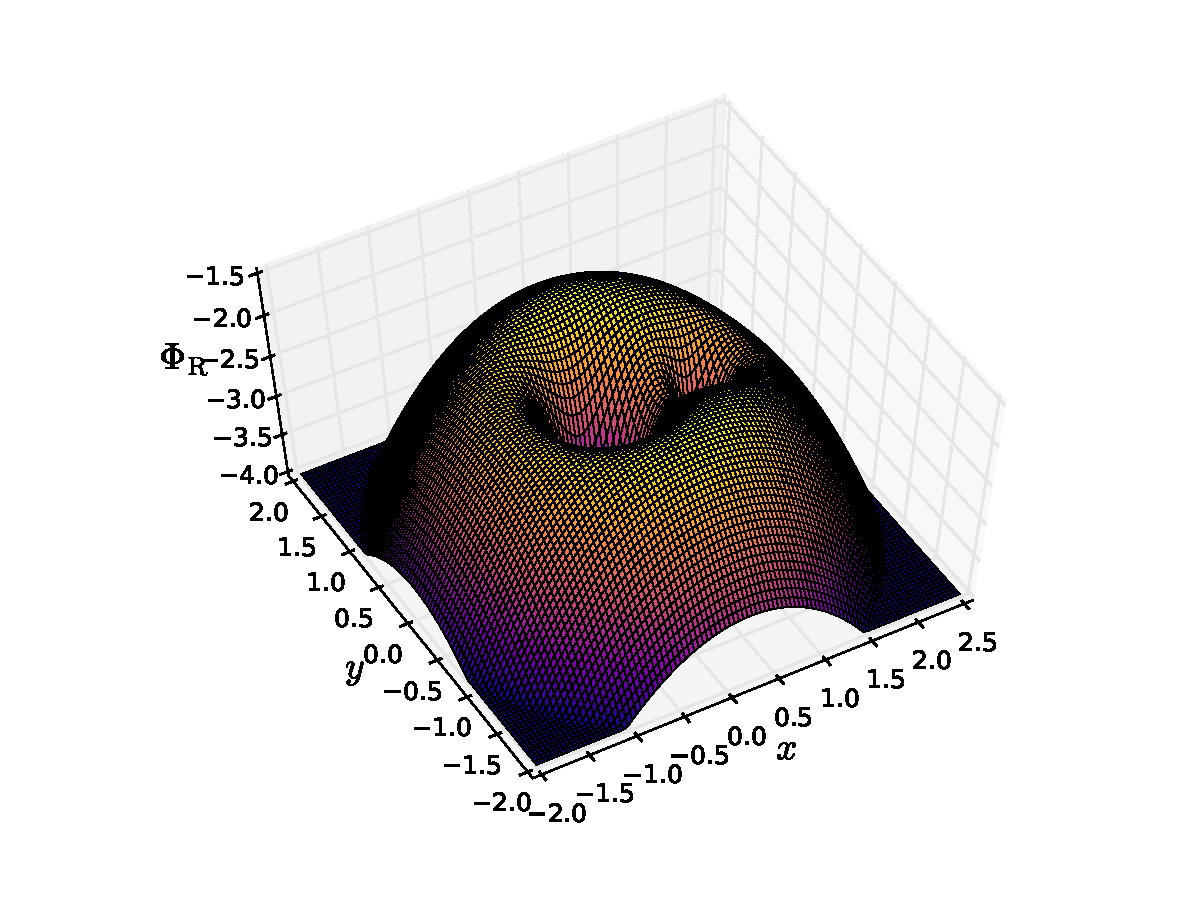
\includegraphics[width=7.5cm]{figs/astro/roche.pdf}
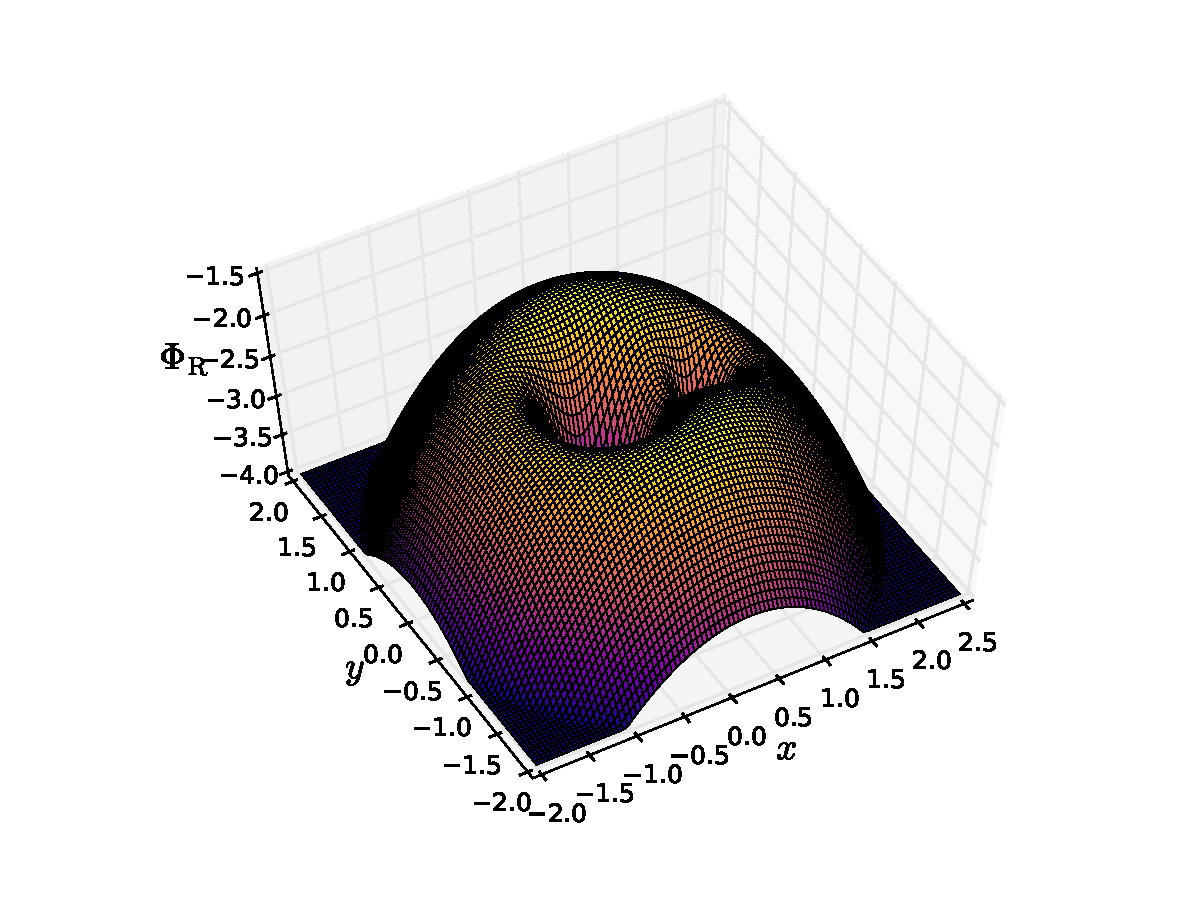
\includegraphics[width=7.5cm]{figs/astro/roche.pdf}
\caption{\label{fig:roche}
Roche potential for binary systems.
}
\end{figure}

\subsubsection{Roche lobes and mass transfer}
Roche Lobe \cite{PRP02} \cite{LL15}

A flow of gas between two stars can be described by the Euler equation.
It gives the time evolution of the velocity $\vec{v}$ of the gas that has a pressure of $P$ and density $\rho$.
In a reference frame rotating together with the binary system with angular velocity $\omega$ the Euler equation takes the form 
\be
\frac{ \partial \vec{v} }{\partial t} + (\vec{v} \cdot \nabla)\vec{v} = -\nabla \Phi_{\mathrm{R}} - 2 \vec{ \omega } \times \vec{v} - \frac{1}{\rho} \nabla P,
\ee
where the angular velocity of the binary is then
\be
\vec{ \omega } = \left( \frac{ G M }{a^3} \right)^{1/2} \vec{e},
\ee
as given with the unit vector $\vec{e}$, normal to the orbital plane.
Here $M$ is the total mass of the system, i.e. $M = M_1 + M_2$, where $M_1$ and $M_2$ are the individual masses of the two stars in the system, respectively, and $a$ is their orbital separation.

The effects originating from the gravitation and from the centrifugal forces are encapsulated in the so-called Roche potential, given as a function of radial vector $\vec{r}$ as
\be
\Phi_{\mathrm{R}}(\vec{r}) = -\frac{G M_1}{|\vec{r} - \vec{r_1}|} -\frac{G M_2}{|\vec{r} - \vec{r_2}|} - \frac{1}{2} ( \vec{ \omega } \times \vec{v} )^2,
\ee
where the location of the stars is given with $\vec{r_1}$ and $\vec{r_2}$.

By studying the shape of the potential, we see that in between the stars, in the so-called $L_1$ point there exists a location where the individual gravitational pull from the stars is balanced.
This leads to a kinda of a nozzle in the system from which the material can leak from the less massive star to the more massive object.
Such a leaking, or a Roche lobe overflow, will then occur if the companion star's radius exceeds the size of its Roche lobe.
Typically such a thing can happen when the star evolves and expands at the end of its life cycle. 

LMXB \cite{TH06}


\subsection{Accretion disks}
Hard and soft state \cite{HvdK89}
Alternates between these two states \cite{MDF14} \cite{DGK07}



\section{Accretion to a neutron star}

\subsection{Boundary layers}

\be
\Omega(R) \approx \Omega_{\mathrm{K}}(R) = \left( \frac{G M}{R^3} \right)^{1/2}
\ee

Layer of thickness $b$ equals $\Omega(R + b) \approx \Omega_{\mathrm{K}}(R + b)$ that must slow down to $\Omega_{*}$.

Energy difference
\be
\dot{E} = \frac{1}{2} \Mdot R^2 (\Omega_{\mathrm{K}}^2 - \Omega_{*}^2) = 
\frac{1}{2} \Mdot \frac{GM}{R} \left[ 1 - \left(\frac{\Omega_*}{\Omega_{\mathrm{K}}} \right)^2 \right] 
\ee

Viscous torque $G_{\mathrm{T}} = \Mdot R^2 (\Omega_{\mathrm{K}} - \Omega_*)$
Hence,
\be
\dot{E} = \frac{1}{2} \frac{G M \Mdot}{R} \left( 1 - \frac{\Omega_*}{\Omega_{\mathrm{K}}} \right)^2
\ee


\subsection{X-ray bursts}
Thermonuclear runaway.

\subsection{Constraining the size of the star}
Cooling tail method.





% --------------------------------------------------
\newpage
\section{Appendix A: Real astrophysics}

%\begin{itemize}
%    \item Accretion
%    \item Disks 
%    \item Soft and hard states
%    \item Boundary layers
%    \item Ignition?
%    \item X-ray bursts
%    \item Cooling tail method
%\end{itemize}
%
%Possible layout:
%
%v1
%\begin{enumerate}
%    \item Accretion
%    \begin{itemize}
%        \item Disks
%        \item Soft and hard states
%        \item Boundary layers
%    \end{itemize}
%    \item X-ray bursts
%    \begin{itemize}
%        \item Unstable thermonuclear burning
%        \item Cooling tail method
%    \end{itemize}
%\end{enumerate}
%
%v2
%\begin{enumerate}
%    \item Accretion disks
%    \begin{itemize}
%        \item Accretion
%        \item ?Roche lobe overflow
%        \item Soft and hard state
%        \item Boundary layers
%    \end{itemize}
%    \item X-ray bursts
%    \begin{itemize}
%        \item Unstable thermonuclear burning
%        \item Cooling tail method
%    \end{itemize}
%\end{enumerate}


\sect{Energetics}
Let us try and estimate the energetics of different phenomena of what we can observe from neutron stars.\mnote{Energy output}
Few possible stable sources of energy exists: thermal, gravitational, rotational, and magnetic.
In addition, unstable fusion processes can also power some observable phenomena.



